\section{Concluding Perspective}
	This Bachelor thesis with the title ``Lexicographic Fréchet Matchings with Degenerate Inputs" discussed three main topics from the Fréchet distance spectrum that build on each other.
	
	First, the classical Fréchet distance as researched by \citeauthor{altgodau} in their \citeyear{altgodau} paper \citetitle{altgodau}\cite{altgodau} is explored. We discussed the free-space diagram, classical critical events of types a, b, and c, and the decision problem.
	
	Second, \citeauthor{rotelex}'s \citeyear{rotelex} paper \citetitle{rotelex}\cite{rotelex} guides us to extend the Fréchet distance to accomplish a lexicographic matching based on the classical Fréchet distance. \citeauthor{rotelex} introduced the steepest descent, a new lexicographic type of critical events, and of course the algorithm for traversing a height function $\delta$ lexicographically.
	
	Third, we investigate lexicographic Fréchet matchings with degenerate inputs based on section 7 of \citeauthor{rotelex}'s paper\cite{rotelex}. The problem of multiple critical events at the same critical height $\epsilon$ is defined and visualised by numerous examples. Through the examples, we discover that two procedures need to be defined. First, we need to know which paths through the critical events are possible and second we need to know which of the paths results in the lexicographically optimal profile to fulfil the goal of a lexicographic traversal.
	
	The problem of degenerate inputs concerning lexicographic Fréchet matchings is by no means solved at this point. The next sections showcase questions that still exist.
	
\subsection{Third, Fourth, Fifth, etc. Derivative}

Equation \ref{eq:hinvd1} defines $[h^{-1}]'(\epsilon)$:

$$[h^{-1}]'(\epsilon) = \frac{ \epsilon }{ a\sqrt{\frac{\epsilon^2 - u^2}{a}} }$$

Due to the square root in the denominator of $[h^{-1}]'(\epsilon)$, $[h^{-1}]'(\epsilon)$ potentially has infinite derivatives.

After taking three derivatives, the values of these three derivatives can be used in an equation system to calculate the three parameters $u$, $a$, and $v$. If we compare two hyperbola inverses, it is enough to compare three derivatives, because if the first three derivatives are the same for two hyperbola inverses, the two hyperbola inverses have the same parameters $u$, $a$, and $v$.

We can extrapolate this to multiple hyperbola inverses: If we are comparing $N$ hyperbola inverses to $N$ other hyperbola inverses, we need to compare at most $3\cdot N$ derivatives, because with $3\cdot N$ derivatives an equation system can be established from which the parameters $u$, $a$, and $v$ can be calculated for each one of the $N$ hyperbola inverses. Therefore the $N$ hyperbolas would be the same. This procedure is only possible for $f$s and $g$s that have the same number $N$ of critical events.

It would be interesting to try to find or construct examples where higher derivatives than the second one are needed. Researching could lead to a proof that only a finite number of derivatives is needed. It might also make sense to look at more derivatives of $h^{-1}(\epsilon)$. See the first five derivatives here:

\begin{align*}
	[h^{-1}]'(\epsilon) &= \frac{ \epsilon }{ a\sqrt{\frac{\epsilon^2 - u^2}{a}} }\\
	[h^{-1}]''(\epsilon) &= -\frac{u^2}{a^2\left(\frac{\epsilon^2 - u^2}{a}\right)^{\frac{3}{2}}}\\
	[h^{-1}]'''(\epsilon) &= \frac{3u^2\epsilon}{a^3\left(\frac{\epsilon^2 - u^2}{a}\right)^{\frac{5}{2}}}\\
	[h^{-1}]''''(\epsilon) &= \frac{3u^2\left(-u^2-4\epsilon^2\right)}{a^4\left(\frac{\epsilon^2 - u^2}{a}\right)^{\frac{7}{2}}}\\
	[h^{-1}]'''''(\epsilon) &= \frac{15u^2\epsilon\left(3u^2+4\epsilon^2\right)}{a^5\left(\frac{\epsilon^2 - u^2}{a}\right)^{\frac{9}{2}}}\\
\end{align*}

	
\subsection{Equal Descents at $\epsilon_0$, Unequal Descents Below}
%https://abegehr.github.io/frechet/?p=(4_5)(8_5.5)(4_6)&q=(5_4)(5_7)(5_4)

In section \ref{sec:ces_min_2} we saw an example where two paths were exactly equal. The example shown in figure \ref{fig:ces_wrong_1} is constructed by slightly mutating the example from section \ref{sec:ces_min_2}.

\begin{figure}[H]
	\centering
    
    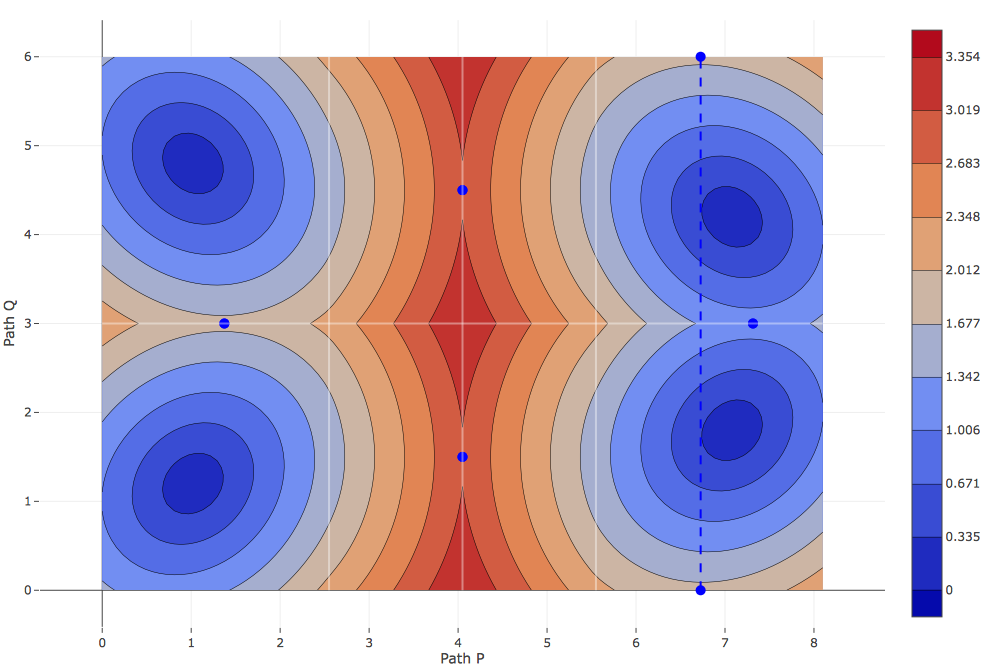
\includegraphics[width=0.7\textwidth]{ces_wrong_1.png}
		
	\caption{Equal descents at $\epsilon_0$, unequal descents below\protect\footnotemark}
    \label{fig:ces_wrong_1}
\end{figure}
\footnotetext{View the example here: \url{https://abegehr.github.io/frechet/?p=(4_5)(6.5_5.5)(8_5.5)(6.5_5.5)(4_6)&q=(5_4)(5_7)(5_4)}\label{ftn:ces_wrong_1}}

The critical height $\epsilon_0 = 3$. There are two critical events: $C_1(4.03, 1.5)$ and $C_2(4.03, 4.5)$. Coordinates are rounded to two decimal places.

There are two paths through the height map $\delta$. One over the classical critical event of type b $C_1(4.03, 1.5)$ and one over the classical critical event of type b $C_2(4.03, 4.5)$.

The hyperbolas representing the ascents to and the descents from $C_1$ and $C_2$ are the same. They contain the same parameters $u$, $a$, and $v$. Therefore both paths are traversed (see figure \ref{fig:ces_wrong_1_tra}).

\begin{figure}[H]
	\centering
    
    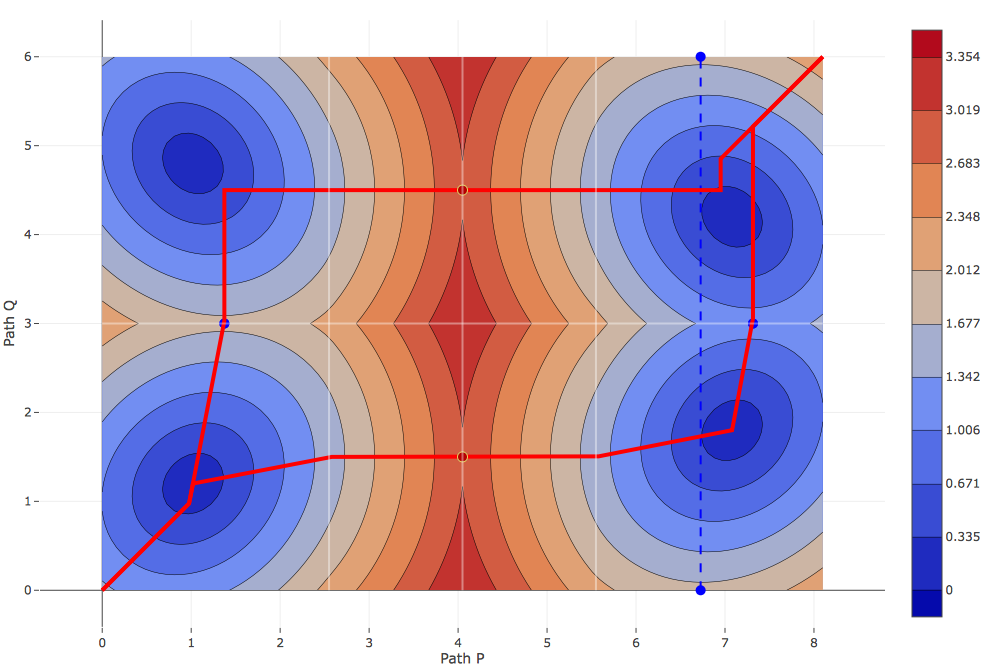
\includegraphics[width=0.8\textwidth]{ces_wrong_1_tra.png}
		
	\caption{Equal descents at $\epsilon_0$, unequal descents below, traversed\textsuperscript{\ref{ftn:ces_wrong_1}}}
    \label{fig:ces_wrong_1_tra}
\end{figure}

At height $\epsilon_0 = 3$ the profiles of both paths are equal, but at $\epsilon_1 \approx 1.765$ the profile of the lower path over $C_1$ turns out to have been the better choice. Figure \ref{fig:ces_wrong_1_csp} shows the cross-sections and profiles of both traversals.

\begin{figure}[H]
	\centering
    
    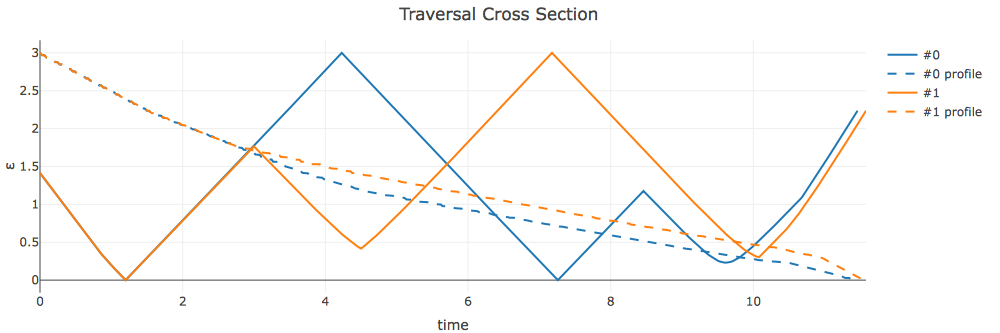
\includegraphics[width=0.7\textwidth]{ces_wrong_1_csp.png}
		
	\caption{Cross-sections and profiles\textsuperscript{\ref{ftn:ces_wrong_1}}}
    \label{fig:ces_wrong_1_csp}
\end{figure}

The traversal \#0 depicts the cross-section and profile for the lower traversal over $C_1$. The traversal \#1 depicts the cross-section and profile for the upper traversal over $C_2$. It can be seen clearly by looking at the cross-sections and profiles of the two traversals that traversing the path over $C_1(4.03, 1.5)$ yields the lexicographically optimal traversal.

The problem is that when the algorithm decides if to traverse $C_1$ or $C_2$, the algorithm does not yet know what happens below $\epsilon_0 = 3$. The algorithm would need to traverse both paths and decide at $\epsilon_1 = 1.765$ which critical event to discard and which critical event to traverse.




